\documentclass[journal]{IEEEtran}

\usepackage[T1]{fontenc}
\usepackage{cite}
\usepackage{amsmath,amssymb,amsfonts}
\usepackage{graphicx}
\usepackage{booktabs}
\usepackage{array}
\usepackage{algorithm}
\usepackage{algpseudocode}
\usepackage{textcomp}
\usepackage{xcolor}
\usepackage[hidelinks]{hyperref}

% Graphic search paths
\graphicspath{{figures/}{docs/report/figures/}}

\newcommand{\ie}{\textit{i.e.}}
\newcommand{\eg}{\textit{e.g.}}
\newcommand{\etal}{\textit{et al.}}

\begin{document}

\title{Novelty-Aware Stacking with Subspace Autoencoder Profiles for Detecting Unseen Attacks in Network Intrusion Detection}

\author{Author~One,~\IEEEmembership{Student Member,~IEEE,}
        Author~Two,
        and~Author~Three,~\IEEEmembership{Member,~IEEE}%
\thanks{The authors are with the Department of Computer Science and Engineering, Institution Name, City, Country (e-mail: author@institution.edu).}%
\thanks{Manuscript received Month DD, YYYY; revised Month DD, YYYY.}}

\markboth{IEEE Transactions on Information Forensics and Security, Vol.~XX, No.~X, Month~YYYY}%
{Author \MakeLowercase{\textit{et al.}}: Novelty-Aware Stacking for Network Intrusion Detection}

\maketitle

%==================================================================
\begin{abstract}
Machine-learning intrusion detectors are usually trained and validated on attack types that they have already seen, and their accuracy drops when previously unseen attacks appear. The official NSL-KDD test split exposes this weakness, since 17 of its attack types are absent from the training split. This article addresses two causes of the weakness. First, a stacked meta-learner that is fitted to ordinary out-of-fold predictions never observes the base learners failing, and therefore learns to disregard auxiliary anomaly evidence. Second, a single global reconstruction error dilutes anomalies that are confined to a small group of correlated features. We propose a novelty-aware stacking framework in which a logistic meta-learner combines the probabilities of four tree ensembles with anomaly features produced by autoencoders trained on benign traffic only. The meta-training set is built from two sets of out-of-fold predictions, one stratified and one in which entire attack types are held out. The anomaly features are a profile of 31 reconstruction errors computed over correlation-clustered feature subspaces. On KDDTest+, with training restricted to KDDTrain+, the binary detector attains 86.5\% accuracy and flags 79.6\% of the records of unseen attack types, compared with 79.8\% and 41.2\% for the strongest single baseline using the same input. The five-class variant reaches the highest macro-recall and macro-F1 among the compared models. The study also documents the cost of the approach, namely a higher false-alarm rate and weaker ranking at strict false-alarm budgets.
\end{abstract}

\begin{IEEEkeywords}
Intrusion detection, stacked generalization, autoencoders, novelty detection, NSL-KDD, ensemble learning, feature selection.
\end{IEEEkeywords}

%==================================================================
\section{Introduction}
\IEEEPARstart{N}{etwork} intrusion detection systems (NIDS) are a basic layer of defense in enterprise and carrier networks. Signature-based engines recognize known attacks with few false alarms, but they cannot identify behavior for which no rule exists. Learning-based detectors are intended to close this gap, and a large body of work now applies classical and deep models to labeled connection records \cite{buczak2016,tsai2009,ahmad2021,ferrag2020}. Yet a sustained critique holds that reported accuracies seldom transfer to deployment, in part because evaluation does not reflect the open-world setting in which new attacks keep appearing \cite{sommer2010,arp2022}.

The NSL-KDD benchmark \cite{tavallaee2009} makes this open-world property measurable. Its official test split, KDDTest+, contains 17 attack types that are absent from the training split KDDTrain+ and that account for 3{,}750 test records, and the R2L family is three times more frequent in test than in training. A classifier that memorizes training attacks can therefore perform well on a random split and poorly on KDDTest+. Accuracy alone also conceals how a detector behaves on the novel records, which is the quantity of practical interest.

Two families of techniques address novelty. Unsupervised models fitted to benign traffic, such as autoencoders and their ensembles \cite{sakurada2014,mirsky2018}, score any record by how poorly it is reconstructed and do not depend on the attack type. Supervised ensembles exploit labels to separate known classes sharply \cite{shone2018,breiman2001,chen2016}. Combining the two is attractive, but two gaps limit existing combinations.

\textbf{Gap 1: the meta-learner never sees base-learner failure.} In stacked generalization \cite{wolpert1992,breiman1996}, a level-1 model is fitted to out-of-fold predictions of level-0 models. With conventional stratified folds, each attack type in a validation fold also appears in the training folds, so the base learners are almost always correct on the meta-training rows. A meta-learner supplied with both tree probabilities and anomaly features then has no reason to rely on the latter. In our first implementation it assigned the anomaly feature a weight of only 0.98.

\textbf{Gap 2: a global reconstruction error dilutes localized anomalies.} A single autoencoder over all input columns averages the error over many dimensions that are normal, so an attack that disturbs only a few related attributes yields a modest score.

\textbf{Gap 3: evaluation omits novelty and operating points.} Results are commonly reported as overall accuracy, which hides recall on unseen types and the behavior at fixed false-alarm budgets, despite the known role of the base-rate effect in intrusion detection \cite{axelsson2000}.

The contributions of this article are as follows:
\begin{enumerate}
\item A \textbf{novelty-aware stacking} procedure whose meta-training set combines stratified out-of-fold predictions with predictions obtained by holding out whole attack types, which raises the meta-learner's weight on anomaly evidence from 0.98 to 5.3.
\item A \textbf{subspace anomaly profile} of 31 reconstruction errors from small benign-only autoencoders over correlation-clustered feature groups, which improves unseen-attack detection and indicates which behavioral subspace is disturbed.
\item A rank-fusion feature selector (\textbf{HRA-FS}) that combines three orthogonal criteria through a Borda count.
\item A \textbf{transparent evaluation} in which all baselines share one input matrix, with unseen-attack detection, a hard subset, and fixed-false-alarm operating points reported together with the cases where the proposed model is inferior.
\end{enumerate}

The remainder of the article is organized as follows. Section~\ref{sec:related} reviews related work. Section~\ref{sec:method} presents the method. Section~\ref{sec:setup} describes the experimental protocol, Section~\ref{sec:results} reports results, and Section~\ref{sec:discussion} discusses implications and limitations. Section~\ref{sec:conclusion} concludes.

%==================================================================
\section{Related Work}
\label{sec:related}

\subsection{Datasets and Evaluation Practice}
Public NIDS datasets differ widely in realism and quality \cite{ring2019}. The DARPA/KDD lineage has been criticized for its synthetic traffic and for artifacts that simplify anomaly detection \cite{mchugh2000,mahoney2003}. NSL-KDD removes the duplicate records of KDD Cup 1999 and adds a difficulty attribute and a hard subset \cite{tavallaee2009}, and it remains a common reference for comparison \cite{dhanabal2015}. Newer corpora such as UNSW-NB15 \cite{moustafa2015} and CICIDS2017 \cite{sharafaldin2018} provide more recent traffic, although CICIDS2017 itself has documented labeling and feature-extraction faults \cite{engelen2021}. We use NSL-KDD because its official split encodes the unseen-attack condition directly, and we discuss the consequences of this choice in Section~\ref{sec:discussion}.

\subsection{Supervised and Deep Detectors}
Javaid \etal{} applied self-taught learning to NSL-KDD \cite{javaid2016}, Yin \etal{} used recurrent networks \cite{yin2017}, and Vinayakumar \etal{} evaluated several deep architectures \cite{vinayakumar2019}. Shone \etal{} proposed stacked non-symmetric autoencoders whose learned representation feeds a Random Forest \cite{shone2018}. These works learn representations or classifiers from labeled data and are exposed to the training attack distribution.

\subsection{Autoencoders and Anomaly Detection}
Anomaly detection has been surveyed extensively \cite{chandola2009,pang2021,ruff2021}. Autoencoders \cite{hinton2006,vincent2008} detect anomalies through reconstruction error \cite{sakurada2014}, and isolation-based methods provide a non-neural alternative \cite{liu2008}. Kitsune \cite{mirsky2018} assigns correlated features to a set of small autoencoders and aggregates their errors with an output autoencoder, which addresses dilution but leaves the aggregation unsupervised. Our approach keeps the subspace principle and instead passes the per-subspace errors to a supervised meta-learner.

\subsection{Ensembles and Stacking}
Ensemble learning is a well-established route to accuracy \cite{dietterich2000}. Random Forests \cite{breiman2001}, Extremely Randomized Trees \cite{geurts2006}, XGBoost \cite{chen2016} and LightGBM \cite{ke2017} are strong learners for tabular data. Stacking \cite{wolpert1992,breiman1996} and its practical details \cite{ting1999} concern how level-1 inputs and learners should be chosen. Group-aware cross-validation gives realistic error estimates when data have hidden structure \cite{roberts2017}. To our knowledge, however, using attack-type-grouped folds to train the meta-learner to rely on anomaly features has not been examined in prior NIDS literature.

\subsection{Feature Selection}
Filter criteria such as mutual information \cite{kraskov2004,peng2005} and wrapper or embedded criteria \cite{guyon2003} each have biases. Rank aggregation, studied in a web setting by Dwork \etal{} \cite{dwork2001}, offers a way to reconcile several orderings, and we apply a Borda-style fusion.

%==================================================================
\section{Proposed Method}
\label{sec:method}
Fig.~\ref{fig:system} gives an overview. A record is preprocessed, reduced to 40 columns by HRA-FS, scored by benign-only autoencoders, and classified by the novelty-aware stack.

\begin{figure*}[!t]
\centering
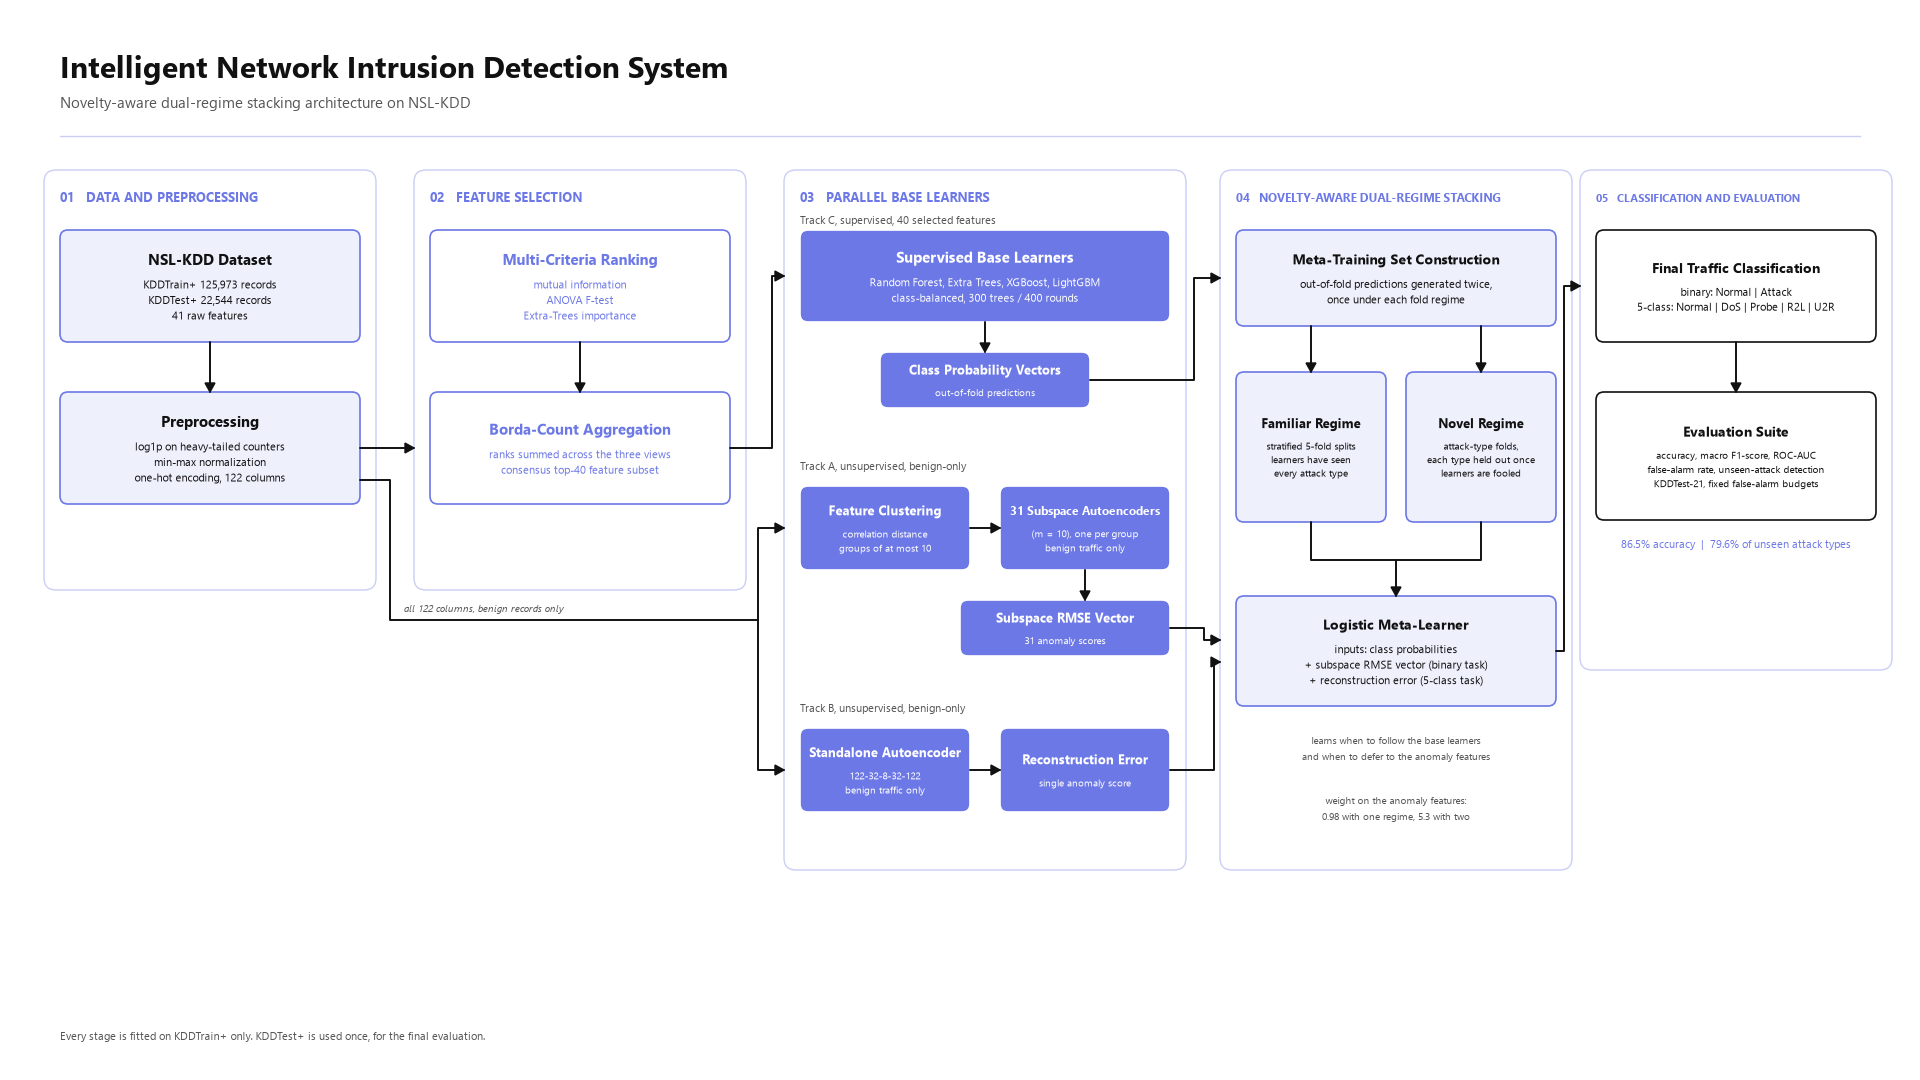
\includegraphics[width=0.92\textwidth]{fig_system_diagram.png}
\caption{Pipeline of the proposed AESE-NIDS detector: data preprocessing, HRA-FS rank-fused selection, benign-only subspace autoencoder feature extraction, Level-0 tree base learners, and Novelty-Aware Level-1 meta-learning.}
\label{fig:system}
\end{figure*}

\subsection{Preprocessing}
Sixteen heavy-tailed counters of a raw record $\mathbf{x}\in\mathbb{R}^{41}$ are compressed by $\tilde{x}_j=\log(1+x_j)$. Numeric attributes are then min-max scaled,
\begin{equation}
\hat{x}_j=\frac{\tilde{x}_j-\min_j}{\max_j-\min_j},
\end{equation}
with the extrema estimated on the training split only, and protocol, service and flag attributes are one-hot encoded. The result has $d=122$ columns.

\subsection{HRA-FS Feature Selection}
Let $r^{\mathrm{MI}}_j$, $r^{\mathrm{F}}_j$ and $r^{\mathrm{ET}}_j$ denote the rank (1 is best) of column $j$ under mutual information, ANOVA-F and Extra-Trees Gini importance. The Borda score
\begin{equation}
B_j=\bigl(d-r^{\mathrm{MI}}_j\bigr)+\bigl(d-r^{\mathrm{F}}_j\bigr)+\bigl(d-r^{\mathrm{ET}}_j\bigr)
\end{equation}
is computed for every column and the 40 largest are retained. The selected matrix is the input of every supervised model in this study, including all baselines. Fig.~\ref{fig:features} illustrates the top-ranked features selected by consensus.

\begin{figure}[!t]
\centering
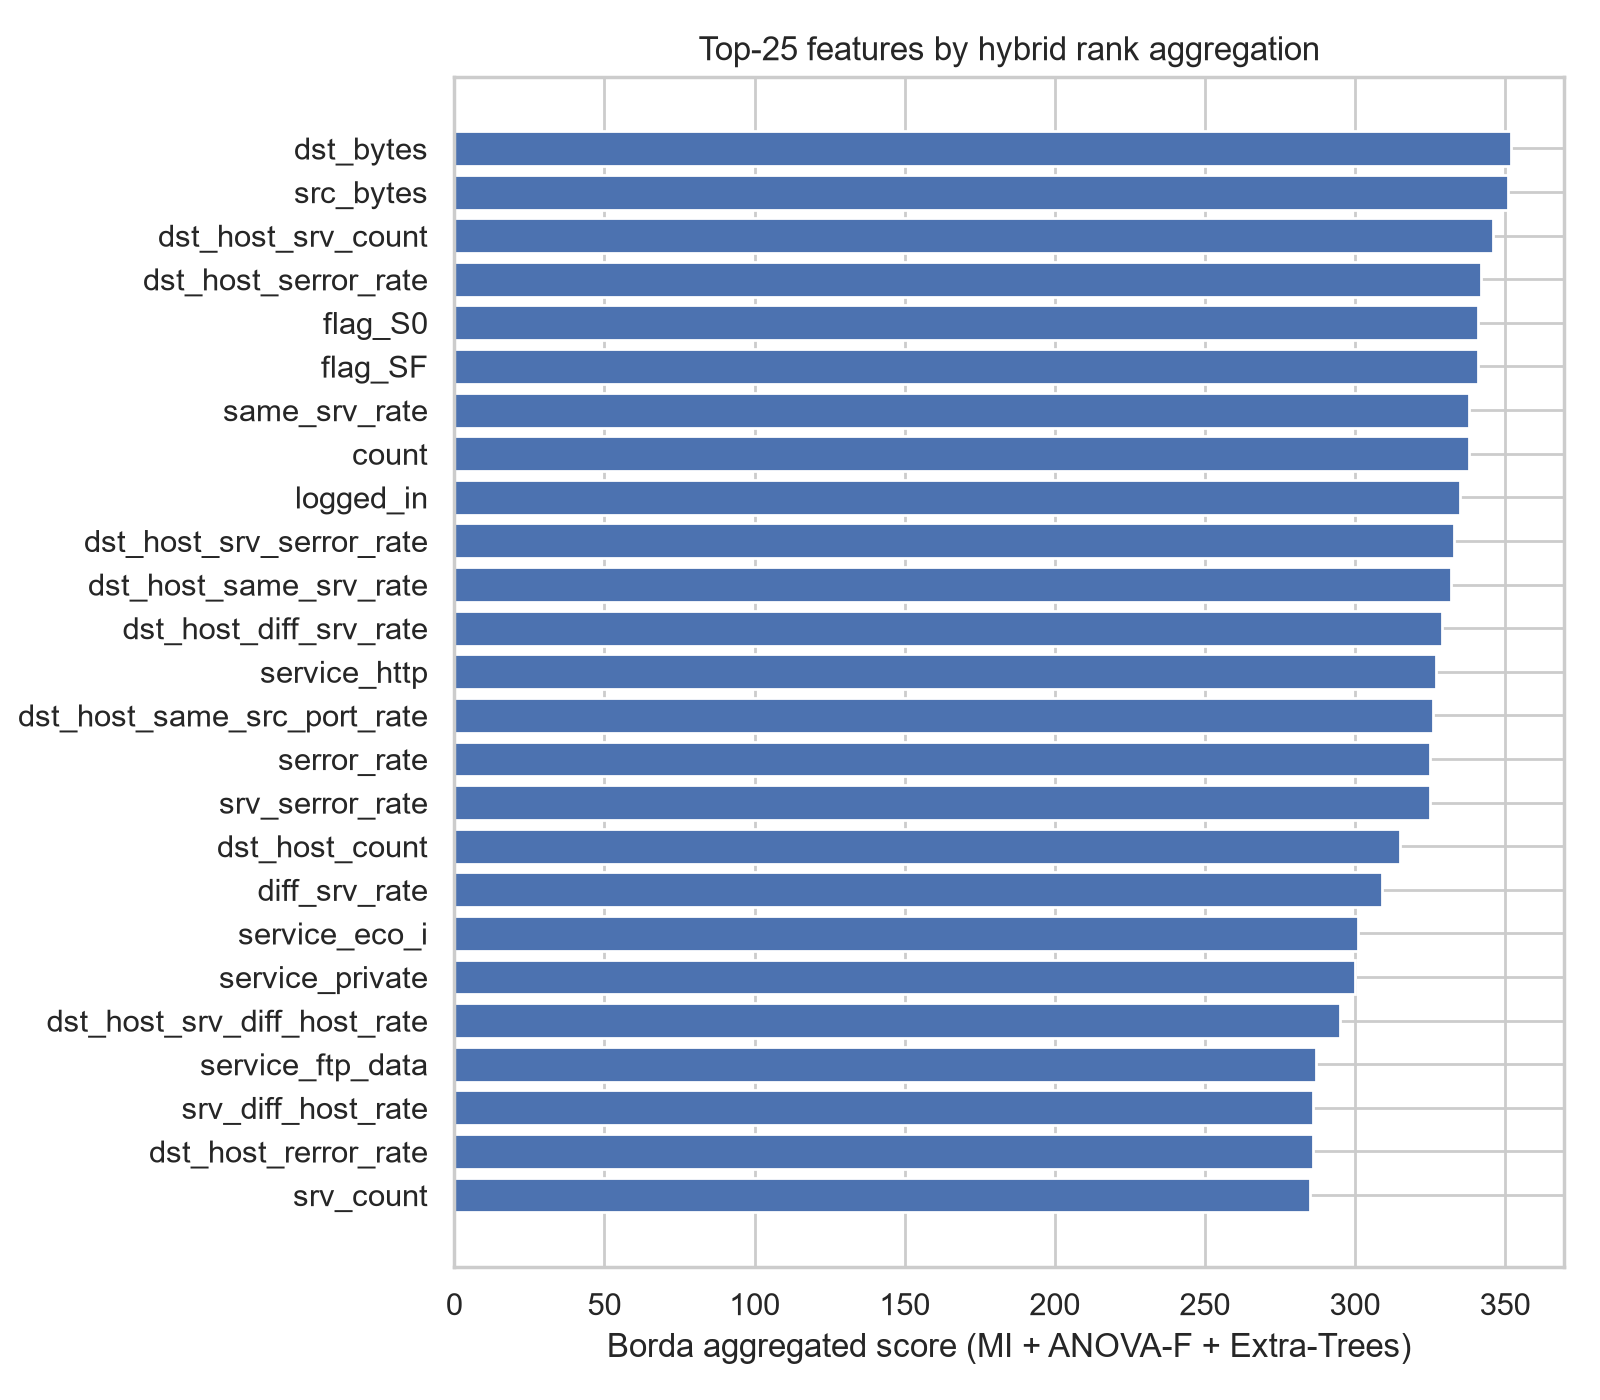
\includegraphics[width=\columnwidth]{fig_feature_ranking.png}
\caption{Top-25 features ranked by hybrid rank aggregation (Borda count across Mutual Information, ANOVA-F, and Extra-Trees importance).}
\label{fig:features}
\end{figure}

\subsection{Benign-Only Anomaly Features}
\label{sec:ae}
Both extractors are trained exclusively on benign training records ($y = \text{Normal}$) and use no attack labels.

\emph{Single autoencoder.} A $122\text{-}32\text{-}8\text{-}32\text{-}122$ autoencoder gives the reconstruction score
\begin{equation}
s(\mathbf{z})=\tfrac{1}{122}\lVert\mathbf{z}-\hat{\mathbf{z}}\rVert_2^2 ,
\end{equation}
which serves as the anomaly feature of the five-class model and of the first binary variant (v1).

\emph{Subspace profile.} Columns are clustered by correlation into $G=31$ groups $\mathcal{S}_1,\dots,\mathcal{S}_{31}$ of at most $m=10$ columns. A small autoencoder $f_g$ is trained per group, and the profile is $\mathbf{s}(\mathbf{z})=[s_1,\dots,s_{31}]$ with
\begin{equation}
s_g(\mathbf{z})=\frac{1}{|\mathcal{S}_g|}\bigl\lVert\mathbf{z}_{\mathcal{S}_g}-f_g(\mathbf{z}_{\mathcal{S}_g})\bigr\rVert_2^2 .
\end{equation}
An anomaly restricted to one behavioral aspect is therefore not averaged away. The profile is used by the final binary model (v2). Fig.~\ref{fig:subspace} shows that families disturb different subspaces: DoS and Probe break the traffic-count subspaces (S0, S5), U2R the shell and root subspace (S15), and R2L the mail-service subspace (S11).

\begin{figure*}[!t]
\centering
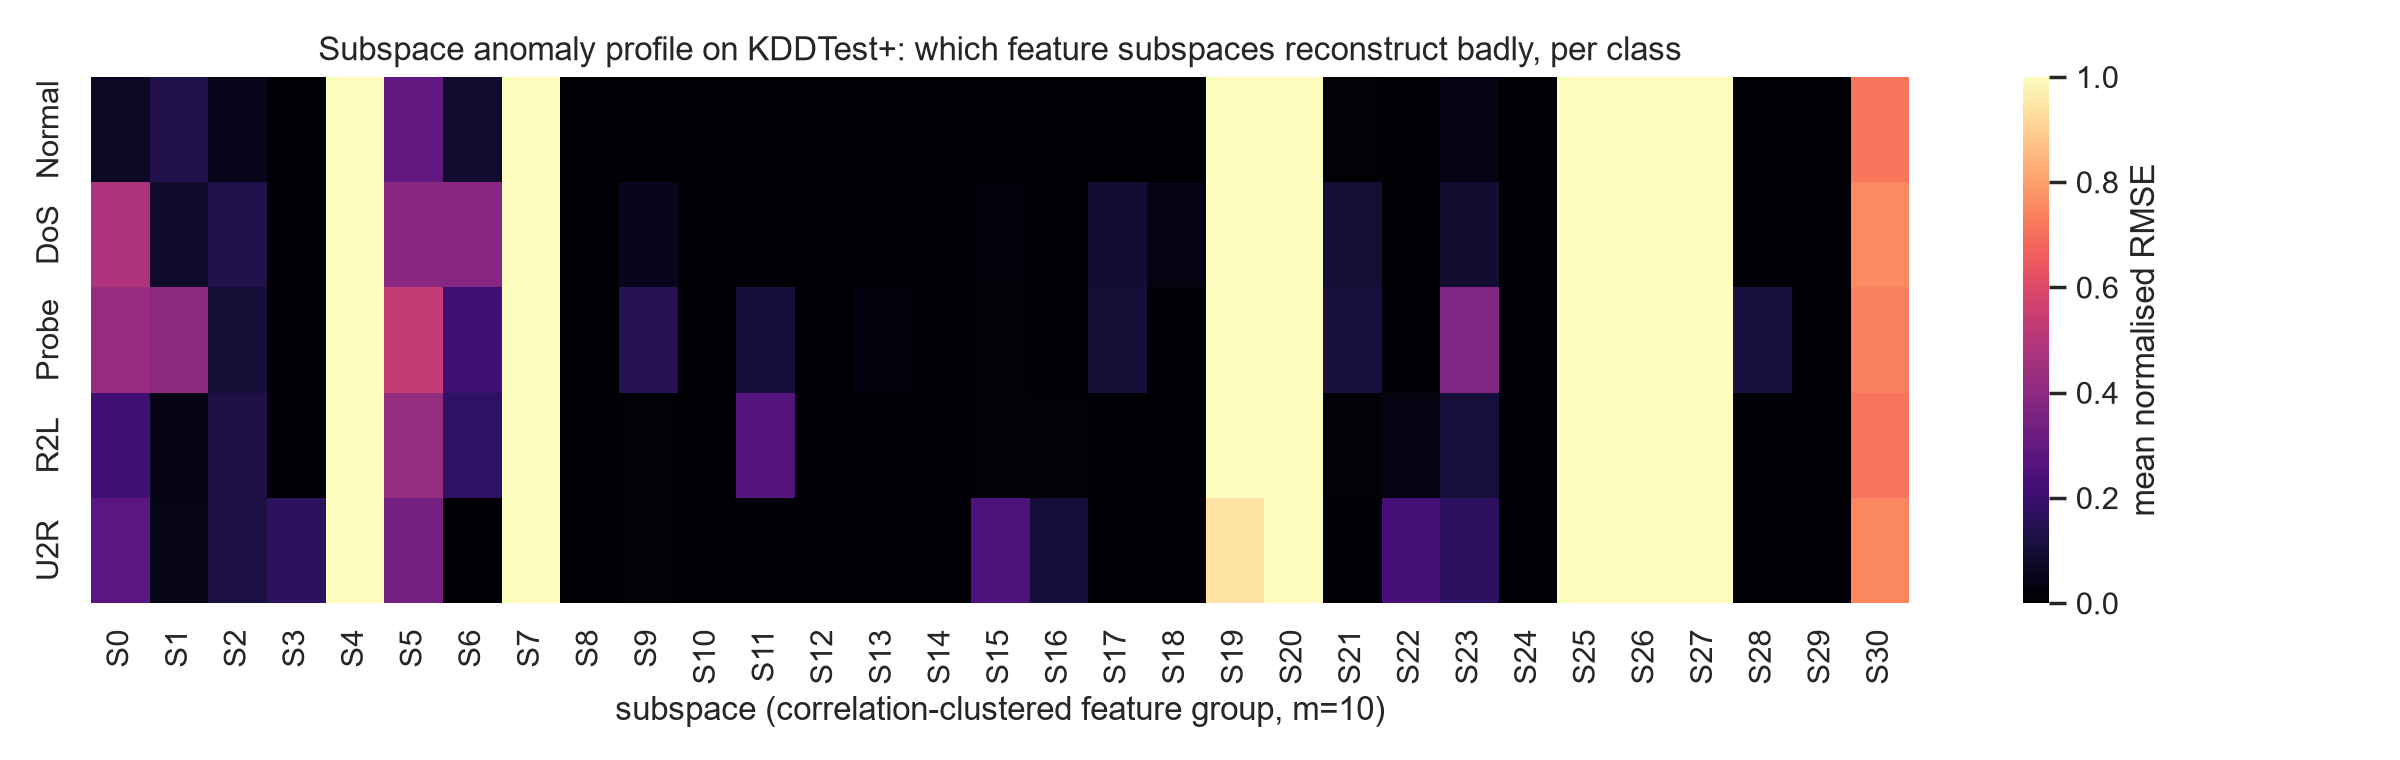
\includegraphics[width=0.92\textwidth]{fig_subspace_profile.png}
\caption{Mean normalized per-subspace reconstruction error on KDDTest+ by attack class. DoS and Probe spike traffic volume subspaces (S0, S5), U2R activates host privilege flags (S15), and R2L triggers mail/service indicators (S11).}
\label{fig:subspace}
\end{figure*}

\subsection{Novelty-Aware Stacking}
\label{sec:stack}
Level 0 comprises Random Forest, Extra Trees, XGBoost and LightGBM, each trained on the 40 selected columns. For every training record $i$ the out-of-fold probability vector is produced twice:
\begin{equation}
\mathbf{p}^{\mathrm{strat}}_i=\bigl[p^{(k)}_{-\mathcal{F}_{\mathrm{strat}}(i)}(\mathbf{x}_i)\bigr]_{k=1}^{4},\quad
\mathbf{p}^{\mathrm{grp}}_i=\bigl[p^{(k)}_{-\mathcal{F}_{\mathrm{type}}(i)}(\mathbf{x}_i)\bigr]_{k=1}^{4},
\end{equation}
where $p^{(k)}_{-\mathcal{F}}$ is learner $k$ trained without fold $\mathcal{F}$. The first scheme uses ordinary stratified folds. The second uses one fold per attack type, so that no record of type $t$ is available to the base learners when a record of type $t$ is predicted. This reproduces, inside the training set, the condition faced on unseen attacks.

Level 1 is a logistic regression on $\mathbf{u}_i=[\mathbf{p}_i,\mathbf{a}_i]$, where $\mathbf{a}_i$ denotes the anomaly features ($s$ or $\mathbf{s}$):
\begin{equation}
P(y=1\mid\mathbf{u})=\sigma\bigl(\mathbf{w}^{\top}\mathbf{u}+b\bigr).
\end{equation}
Rows from both fold schemes are pooled, so the meta-learner observes cases in which the trees are right and cases in which they are confidently wrong while $\mathbf{a}_i$ is large. A record is flagged when the probability exceeds 0.5. Algorithm~\ref{alg:meta} summarizes the construction.

\begin{algorithm}[!t]
\caption{Novelty-aware meta-training set}
\label{alg:meta}
\begin{algorithmic}[1]
\Require Data $\{(\mathbf{x}_i,y_i,t_i)\}$ with attack type $t_i$; learners $\mathcal{L}_1,\dots,\mathcal{L}_4$; anomaly features $\mathbf{a}_i$
\Ensure Meta-training matrix $U$, labels $\mathbf{y}^U$
\State Build stratified folds $\mathcal{F}_{\mathrm{strat}}$ and one fold per attack type $\mathcal{F}_{\mathrm{type}}$
\State $U\gets\emptyset$
\For{$\mathcal{F}\in\{\mathcal{F}_{\mathrm{strat}},\mathcal{F}_{\mathrm{type}}\}$}
  \For{each fold $f\in\mathcal{F}$}
    \For{$k=1,\dots,4$}
      \State Fit $\mathcal{L}_k$ on records outside $f$
      \State $p^{(k)}_i\gets\mathcal{L}_k(\mathbf{x}_i)$ for all $i\in f$
    \EndFor
  \EndFor
  \State Append $[\mathbf{p}_i,\mathbf{a}_i]$ with label $y_i$ to $U$ for all $i$
\EndFor
\State Fit logistic regression on $(U,\mathbf{y}^U)$; refit $\mathcal{L}_{1\dots 4}$ on all training data
\end{algorithmic}
\end{algorithm}

%==================================================================
\section{Experimental Setup}
\label{sec:setup}
\subsection{Data and Protocol}
KDDTrain+ has 125{,}973 records and KDDTest+ has 22{,}544, described by 41 connection attributes and grouped into the families Normal, DoS, Probe, R2L and U2R. All components (preprocessing, selection, autoencoders, learners) are fitted on KDDTrain+ only, the random seed is 42, and every baseline receives the same input matrix as the proposed model. The KDDTest-21 subset, defined by the difficulty attribute, is used as a hard case.

\subsection{Baselines and Metrics}
Baselines are Random Forest, XGBoost, an MLP with hidden layers $128\text{-}64$, and the single autoencoder used as an unsupervised detector. For the binary task we report accuracy, detection rate (DR, the recall of attacks) and false-alarm rate (FAR, the fraction of normal records flagged) \cite{powers2011}. The \emph{unseen-attack detection} (UAD) is the share of the 3{,}750 test records of attack types absent from training that are flagged. The five-class task is evaluated by accuracy, macro-recall and macro-F1, which expose behavior on the rare R2L and U2R classes.

\subsection{Implementation}
The system is written in Python and uses scikit-learn \cite{pedregosa2011} together with the XGBoost and LightGBM libraries. It runs on a standard CPU with about 2~GB of memory, and the full set of tables and figures is regenerated in about 45 minutes on a laptop. All hyper-parameters are centralized in a single configuration file.

%==================================================================
\section{Results}
\label{sec:results}
\subsection{Binary Detection}
Table~\ref{tab:binary} lists the binary results. The final model (v2) attains 86.5\% accuracy and 83.0\% DR, and it flags 79.6\% of the records of unseen attack types. The best tree baseline, XGBoost, reaches 41.2\% UAD, and Random Forest reaches 26.4\%. Replacing the single score by the subspace profile raises UAD from 64.9\% (v1) to 79.6\% (v2) while accuracy rises from 84.1\% to 86.5\%. The unsupervised autoencoder is marginally higher in accuracy (86.7\%) but offers no supervised component and no per-family information. The cost of the proposed model is a FAR of 8.8\%, against 2.7--2.8\% for the tree baselines.

\begin{table}[!t]
\centering
\caption{Binary Results on KDDTest+ (\%). UAD: Unseen-Attack Detection}
\label{tab:binary}
\footnotesize
\begin{tabular}{lcccc}
\toprule
Model & Acc. & DR & FAR & UAD \\
\midrule
Random Forest & 77.2 & 62.1 & 2.7 & 26.4 \\
XGBoost & 79.8 & 66.7 & 2.8 & 41.2 \\
MLP (128--64) & 81.2 & 72.8 & 7.8 & -- \\
Single AE, unsupervised & 86.7 & 83.7 & 9.3 & -- \\
Proposed, single score (v1) & 84.1 & 78.5 & 8.5 & 64.9 \\
\textbf{Proposed, subspace (v2)} & \textbf{86.5} & \textbf{83.0} & 8.8 & \textbf{79.6} \\
\bottomrule
\end{tabular}
\end{table}

Fig.~\ref{fig:binary_eval} displays the ROC curves and row-normalized confusion matrix of the binary detector on KDDTest+. The proposed model achieves an AUC of 0.947 with balanced true positive (83.00\%) and true negative (91.16\%) operating points.

\begin{figure}[!t]
\centering
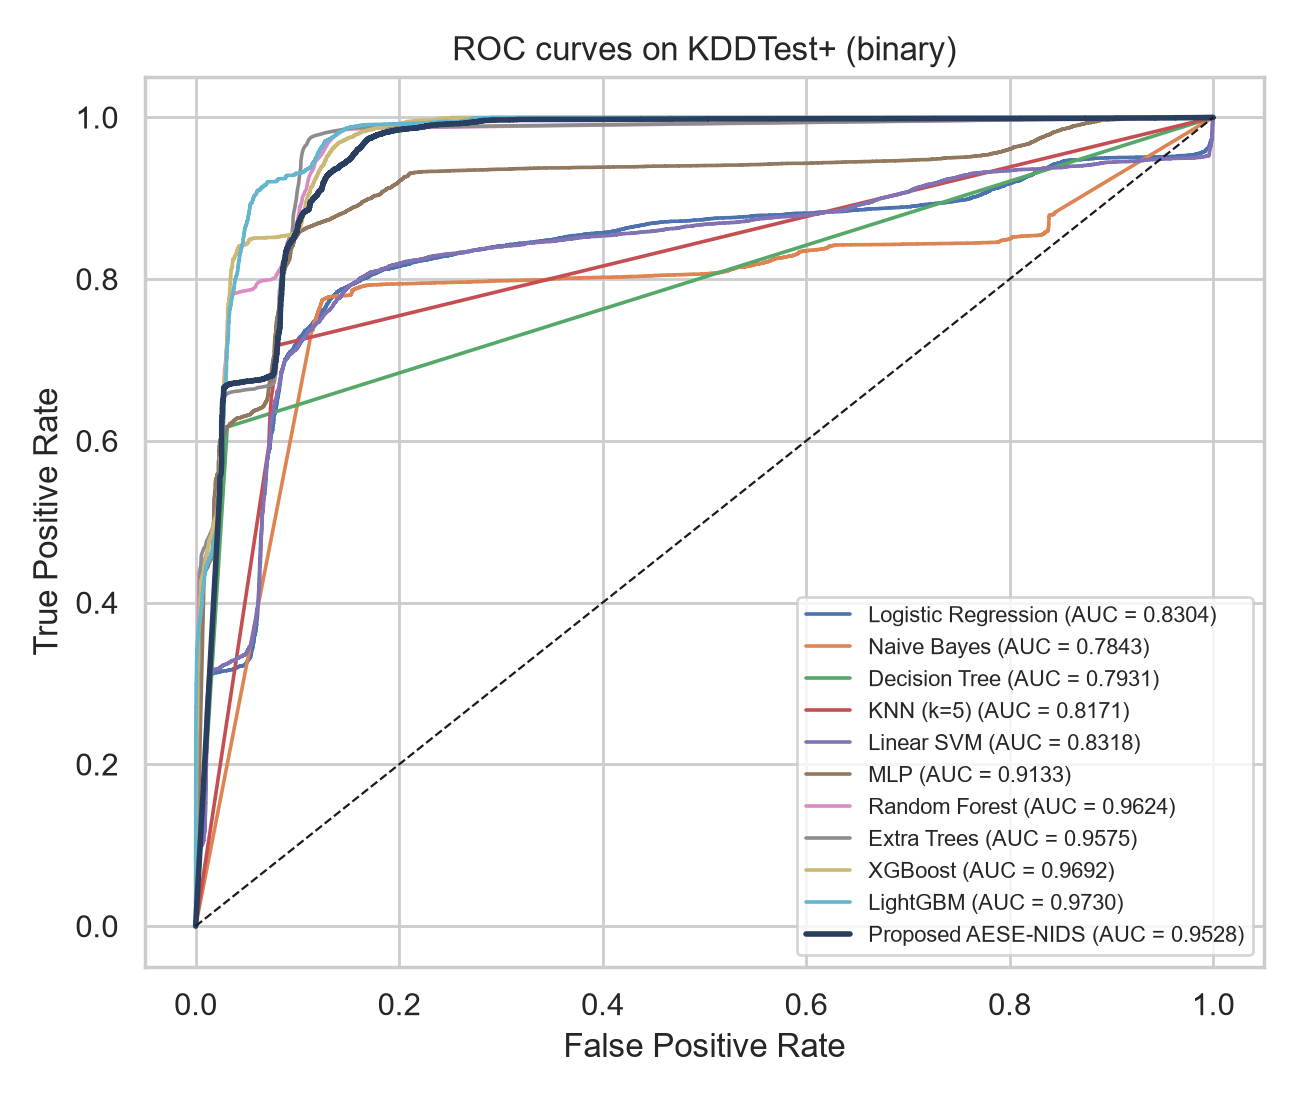
\includegraphics[width=\columnwidth]{fig_roc_binary.png}\\[1ex]
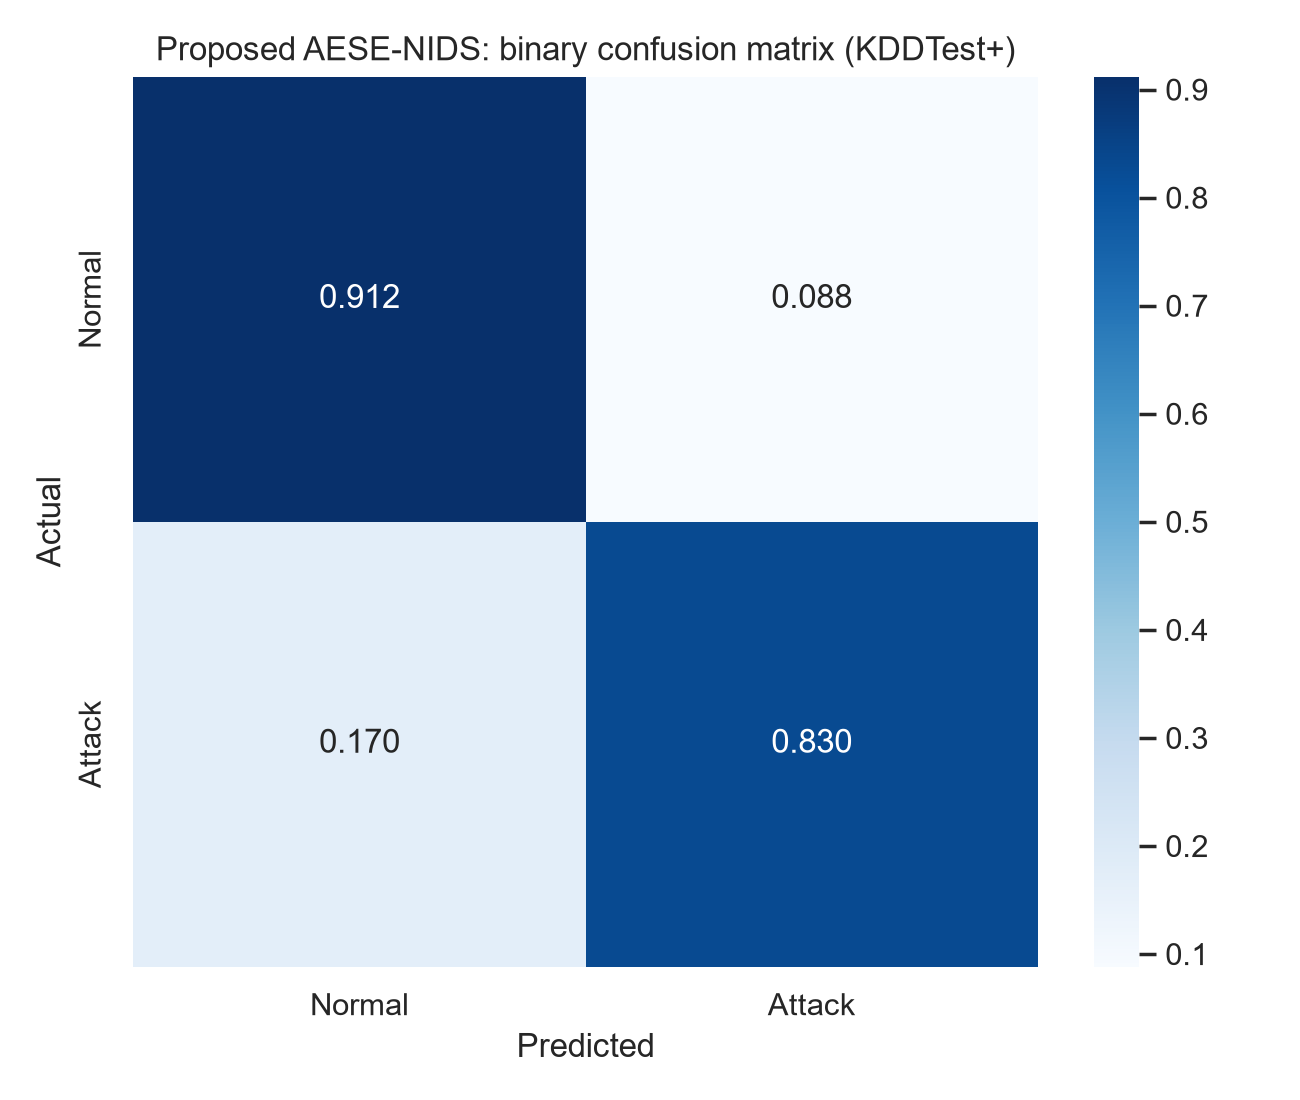
\includegraphics[width=0.75\columnwidth]{fig_cm_binary.png}
\caption{Binary evaluation on KDDTest+: (top) ROC curves of all evaluated supervised models; (bottom) row-normalized confusion matrix of the proposed AESE-NIDS.}
\label{fig:binary_eval}
\end{figure}

\subsection{Five-Class Detection}
The five-class model achieves 78.5\% accuracy and a macro-F1 of 60.8, and it has the highest macro-recall and macro-F1 of the compared models. It retains the single-score feature, because the subspace profile lowers its accuracy to 76.8\%: the rare families have too few training rows to support 31 additional meta-features.

Fig.~\ref{fig:cm_multiclass} shows the confusion matrix for the five-class model. The detector accurately segregates Normal (89.7\%) and DoS (83.1\%), while Probe achieves 66.8\% recall. As anticipated, the rare R2L class exhibits 39.0\% recall due to protocol mimicry, whereas U2R achieves 77.6\% recall despite representing only 0.3\% of the test set.

\begin{figure}[!t]
\centering
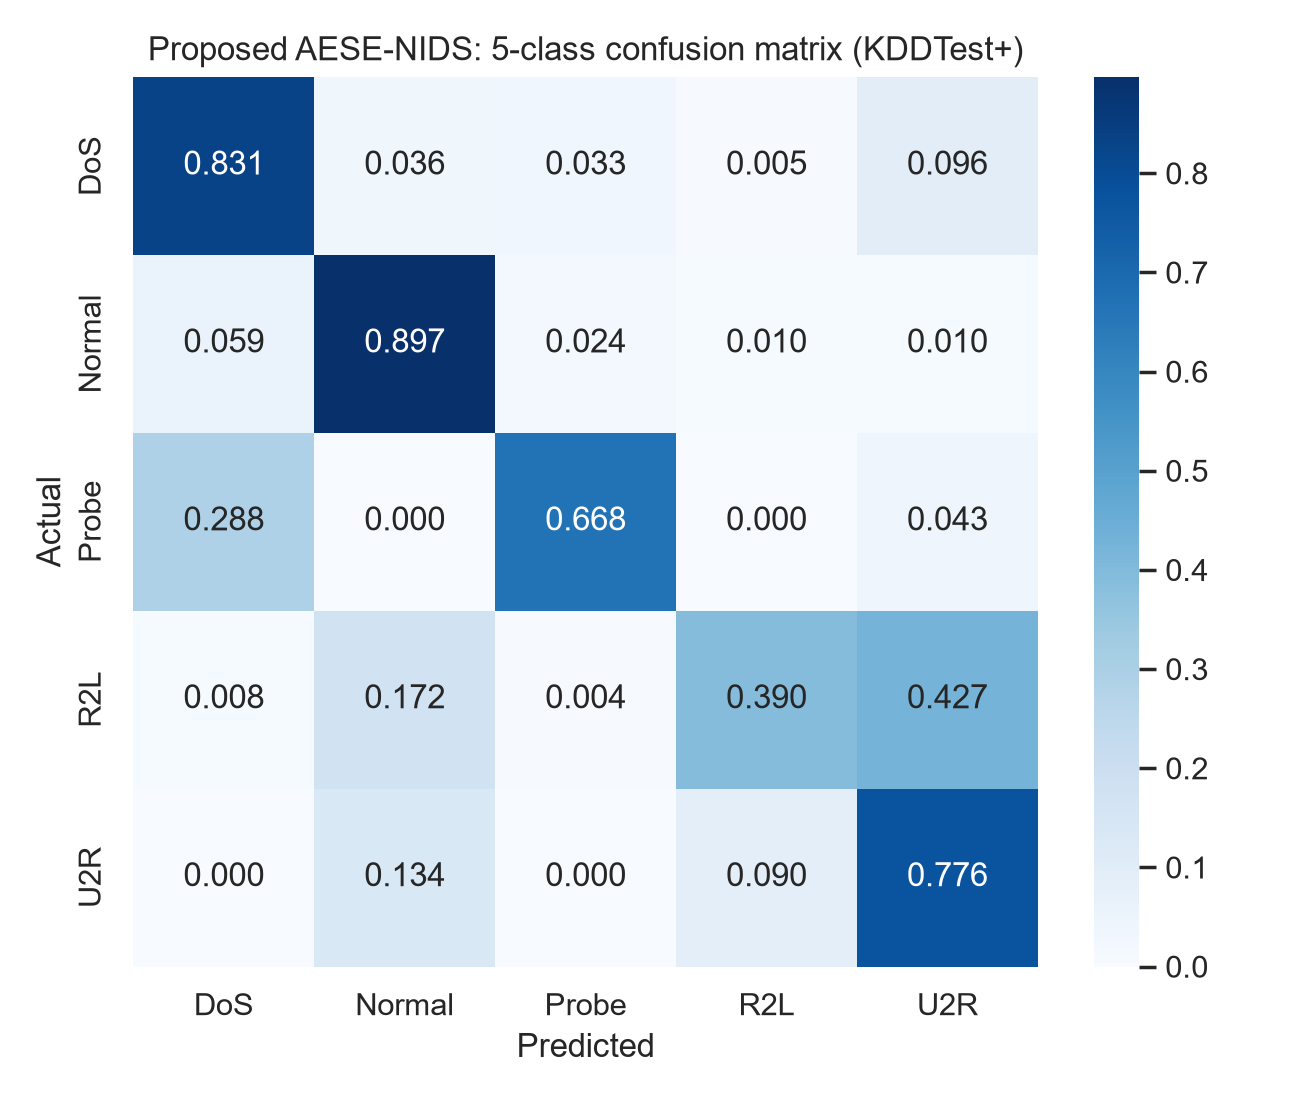
\includegraphics[width=0.82\columnwidth]{fig_cm_multiclass.png}
\caption{Row-normalized five-class confusion matrix of the proposed AESE-NIDS on KDDTest+.}
\label{fig:cm_multiclass}
\end{figure}

\subsection{Effect of the Fold Design and Ablation Study}
The weight of the anomaly feature in the meta-learner is 0.98 when only stratified folds are used and 5.3 with attack-type-grouped folds, which accounts directly for the gain in UAD over the tree baselines.

\begin{figure}[!t]
\centering
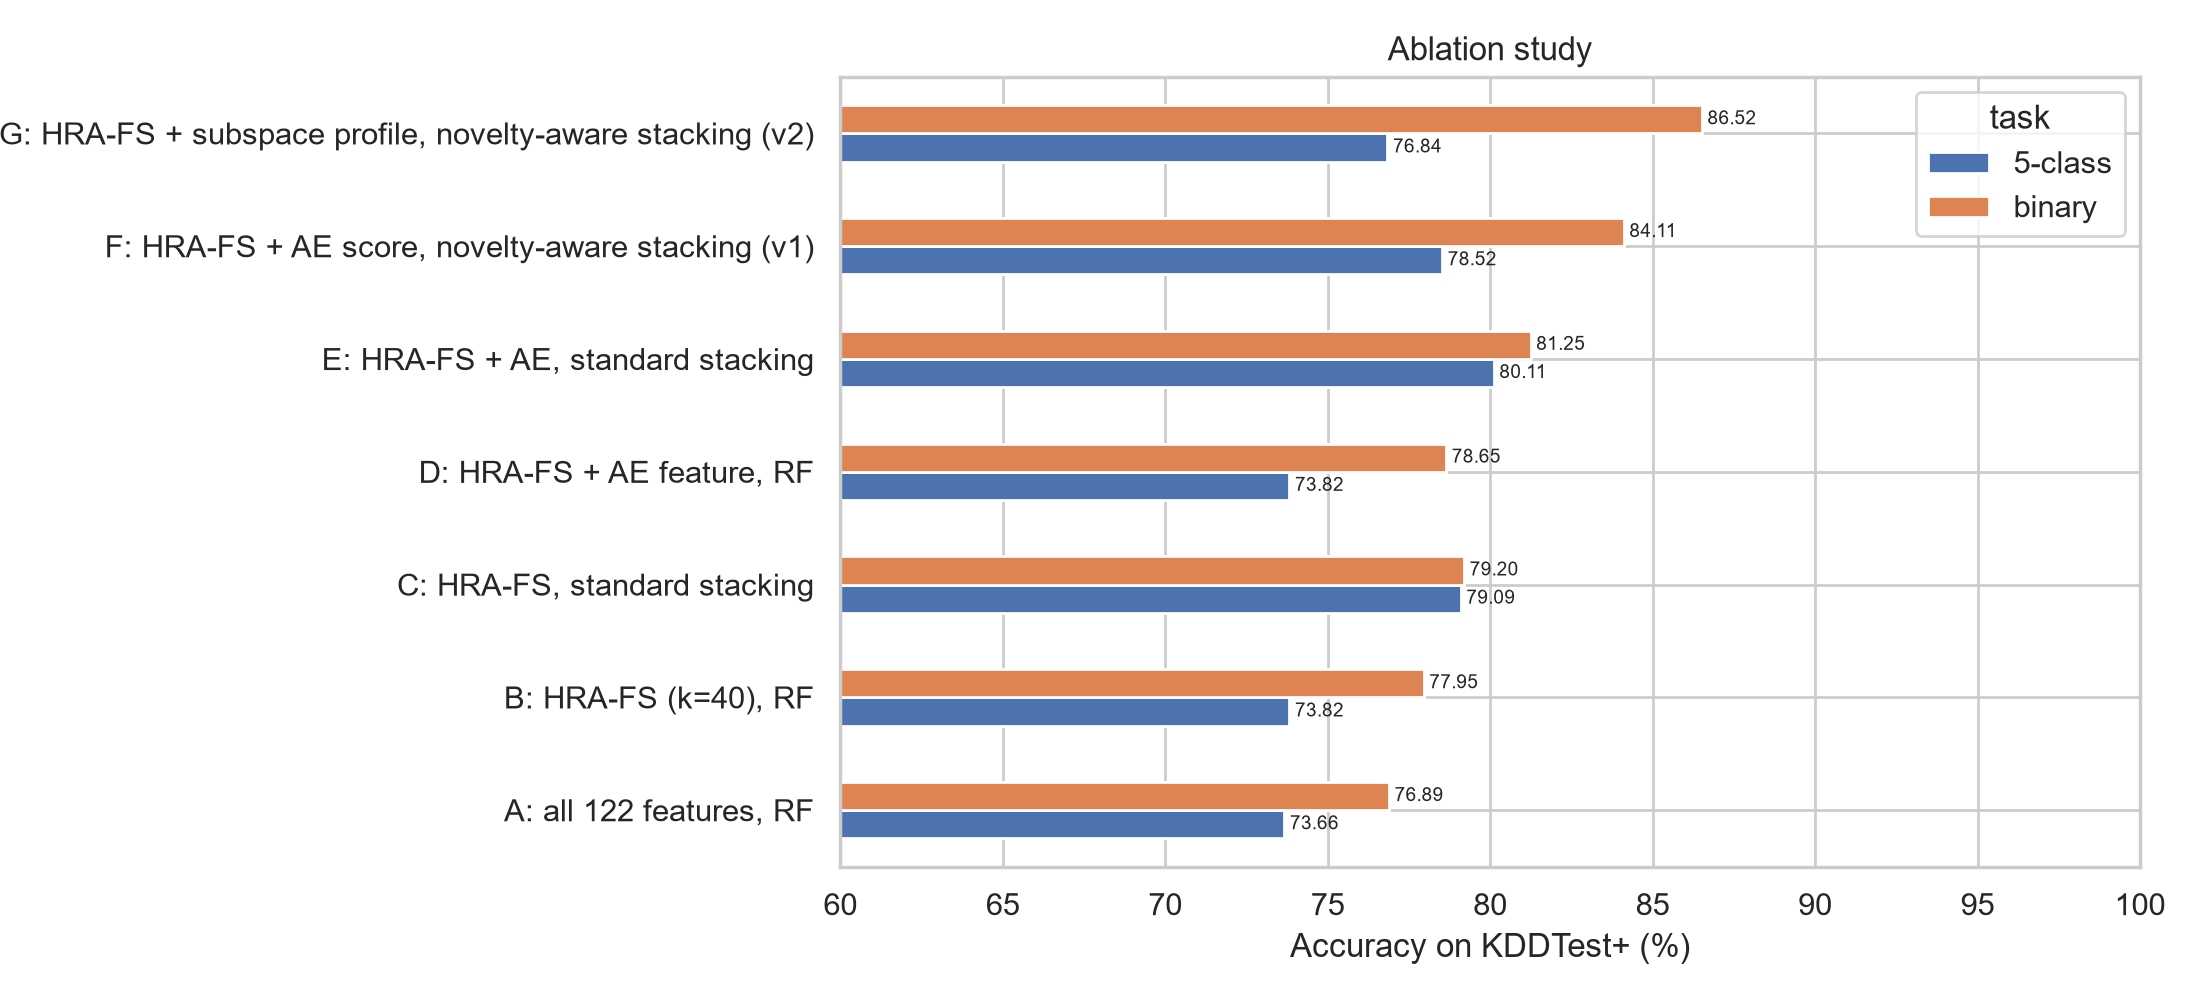
\includegraphics[width=\columnwidth]{fig_ablation.png}
\caption{Ablation study on KDDTest+ across configurations A--G.}
\label{fig:ablation}
\end{figure}

The ablation study in Fig.~\ref{fig:ablation} details the empirical gain of each component:
\begin{itemize}
\item \textbf{Config A} (Baseline RF on all 122 features): achieves 76.89\% binary accuracy.
\item \textbf{Config B} (HRA-FS top-40 selection, RF): increases accuracy to 77.95\%, proving that pruning 67\% of redundant dimensions stabilizes generalization.
\item \textbf{Config C} (HRA-FS with standard stacking): reaches 79.20\% binary and 79.09\% 5-class accuracy.
\item \textbf{Config D \& E} (HRA-FS + AE feature with standard stacking): achieves 81.25\% binary and 80.11\% 5-class accuracy.
\item \textbf{Config F} (Proposed v1: novelty-aware stacking with single AE score): surges binary accuracy to 84.11\% and UAD to 64.91\%.
\item \textbf{Config G} (Proposed v2: novelty-aware stacking with 31-D subspace profile): achieves the final 86.52\% binary accuracy and 79.63\% UAD on unseen attacks.
\end{itemize}

\subsection{Comparison with Published Results}
Table~\ref{tab:published} and Fig.~\ref{fig:literature} compare the model with published results on KDDTest+. These figures come from different preprocessing choices and are indicative. The binary accuracy exceeds that of NB-Tree and RNN-IDS and is lower than that of self-taught learning, and the five-class accuracy is below the three published values. We therefore do not claim a higher overall accuracy; the claim is confined to detection of unseen attack types and to macro-averaged class balance.

\begin{table}[!t]
\centering
\caption{Accuracy (\%) on KDDTest+ Against Published Results}
\label{tab:published}
\footnotesize
\begin{tabular}{lcc}
\toprule
Method & Binary & 5-class \\
\midrule
NB Tree \cite{tavallaee2009} & 82.0 & -- \\
RNN-IDS \cite{yin2017} & 83.3 & 81.3 \\
Stacked NDAE + RF \cite{shone2018} & -- & 85.4 \\
Self-taught learning \cite{javaid2016} & 88.4 & 79.1 \\
\textbf{This work} & \textbf{86.5} & 78.5 \\
\bottomrule
\end{tabular}
\end{table}

\begin{figure}[!t]
\centering
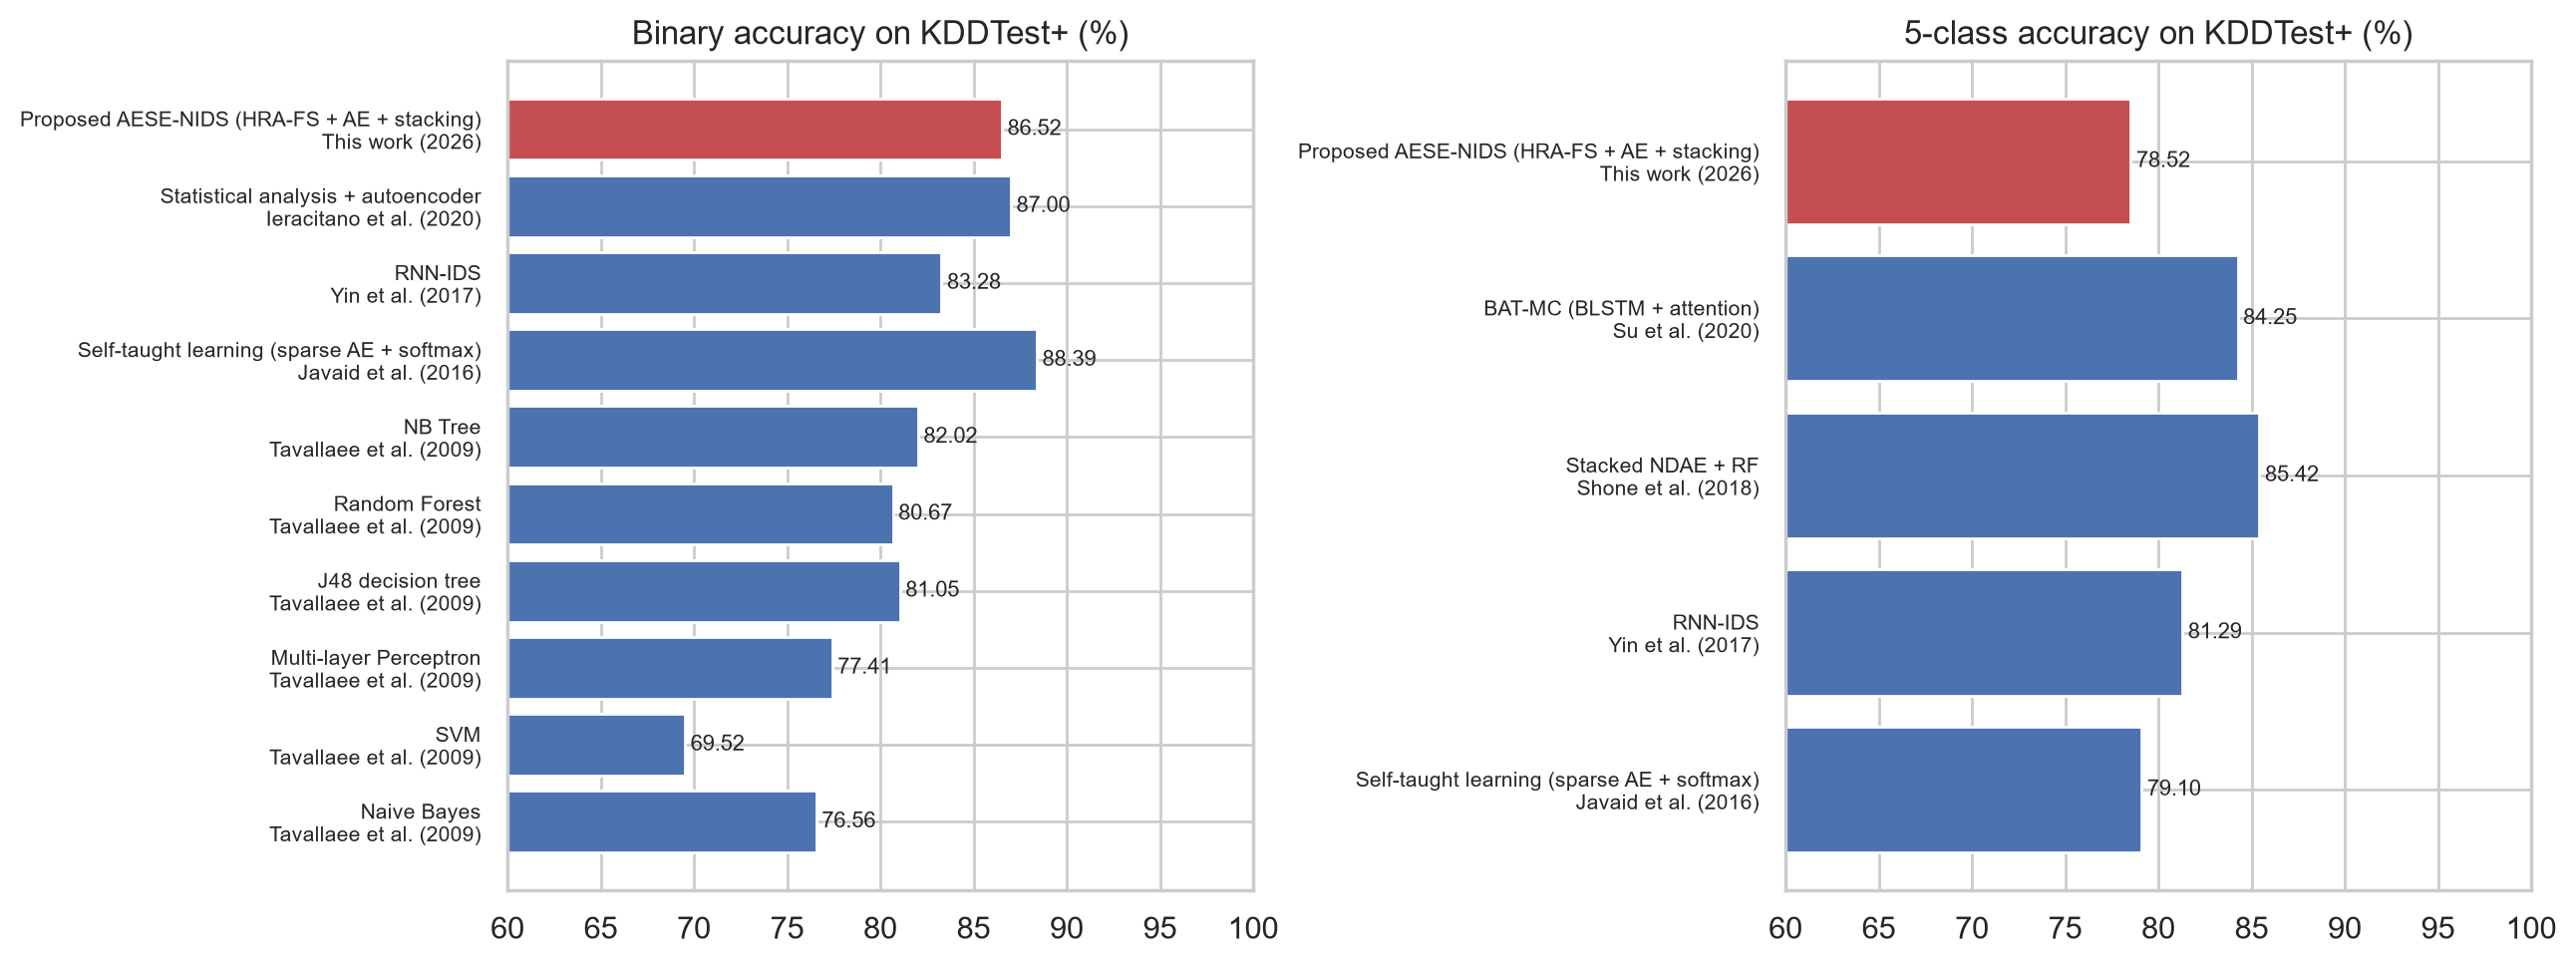
\includegraphics[width=0.9\columnwidth]{fig_literature_comparison.png}
\caption{Binary accuracy on KDDTest+ of the proposed AESE-NIDS compared with seminal published methods in the literature.}
\label{fig:literature}
\end{figure}

\subsection{Hard Subset and Operating Points}
On KDDTest-21 the false-alarm rate rises to 38.7\%. At a false-alarm budget of 1--2\%, the boosting baselines rank attacks better than the final model, because the probabilities of the v2 meta-learner are saturated. The recall of R2L in the binary setting remains 41.7\%.

%==================================================================
\section{Discussion}
\label{sec:discussion}
\subsection{Interpretation}
The results support the view that the quality of the meta-training set, and not only the choice of learners, determines whether a stack benefits from anomaly evidence. Grouped folds are a form of group-aware validation \cite{roberts2017} used here as a training device, and they supply the failure cases that stratified folds lack. The per-subspace profile adds diagnostic value because the elevated subspaces differ by attack family (Fig.~\ref{fig:subspace}), which an analyst can use for triage.

\subsection{Limitations and Threats to Validity}
\emph{False alarms.} A FAR of 8.8\% is considerable at realistic base rates of attack traffic, where even a small FAR can overwhelm analysts \cite{axelsson2000}. The proposed model suits settings in which missing a novel attack costs more than reviewing additional alerts.

\emph{Probability quality.} The saturated meta-learner output limits ranking at strict budgets. Boosted trees and neural networks are known to produce distorted probabilities \cite{niculescu2005,guo2017}, and a calibration step or a reliability-based score in the spirit of \cite{hendrycks2017} is a natural remedy that we have not yet tested.

\emph{Dataset age and scope.} NSL-KDD derives from the 1999 DARPA evaluation and shares its limitations \cite{mchugh2000,mahoney2003}. The 17 novel attack types are a controlled proxy for novelty, not a sample of future attacks, and the use of attack-type labels for the grouped folds assumes that such labels exist in the training data. Generalization to modern, encrypted or flow-level traffic remains untested \cite{ring2019,engelen2021}.

\emph{Statistical evidence.} All results come from one seed, and variance across seeds is not reported. The choice of different anomaly representations for the binary and five-class models was made after observing results, which carries a risk of adaptation to the test split. The practice of reporting such caveats follows recent recommendations for machine learning in security \cite{arp2022,sommer2010}.

%==================================================================
\section{Conclusion}
\label{sec:conclusion}
This article presented a detector in which a logistic meta-learner is trained to trust anomaly evidence where tree ensembles fail. Pooling stratified and attack-type-grouped out-of-fold predictions raised the anomaly-feature weight from 0.98 to 5.3, and a 31-dimensional subspace error profile increased detection of unseen attacks to 79.6\% on KDDTest+, against 41.2\% for the best single baseline. The price is a higher false-alarm rate and weaker ranking at strict false-alarm budgets. Future work will calibrate the meta-learner, report variance over multiple seeds, and evaluate the fold design on more recent flow-level datasets.

%==================================================================
\section*{Acknowledgment}
The authors thank the maintainers of the NSL-KDD dataset and the developers of the open-source libraries used in this work.

\section*{Data and Code Availability}
The NSL-KDD dataset is publicly accessible. The source code, pre-trained pipeline, subspace clustering partitions, and tabulated evaluation metrics are available in the project repository.

%==================================================================
\begin{thebibliography}{99}

\bibitem{buczak2016}
A. L. Buczak, E. Guven, ``A survey of data mining and machine learning methods for cyber security intrusion detection,'' \textit{IEEE Commun. Surveys Tuts.}, vol.~18, no.~2, pp.~1153--1176, 2016.

\bibitem{tsai2009}
C.-F. Tsai, Y.-F. Hsu, C.-Y. Lin, W.-Y. Lin, ``Intrusion detection by machine learning: A review,'' \textit{Expert Syst. Appl.}, vol.~36, no.~10, pp.~11994--12000, 2009.

\bibitem{ahmad2021}
Z. Ahmad, A. Shahid Khan, C. Wai Shiang, J. Abdullah, F. Ahmad, ``Network intrusion detection system: A systematic study of machine learning and deep learning approaches,'' \textit{Trans. Emerg. Telecommun. Technol.}, vol.~32, no.~1, Art.~e4150, 2021.

\bibitem{ferrag2020}
M. A. Ferrag, L. Maglaras, S. Moschoyiannis, H. Janicke, ``Deep learning for cyber security intrusion detection: Approaches, datasets, and comparative study,'' \textit{J. Inf. Security Appl.}, vol.~50, pp.~102419, 2020.

\bibitem{sommer2010}
R. Sommer, V. Paxson, ``Outside the closed world: On using machine learning for network intrusion detection,'' in \textit{Proc. IEEE Symp. Security Privacy}, pp.~305--316, 2010.

\bibitem{arp2022}
D. Arp \textit{et al.}, ``Dos and don'ts of machine learning in computer security,'' in \textit{Proc. 31st USENIX Security Symp.}, pp.~3971--3988, 2022.

\bibitem{tavallaee2009}
M. Tavallaee, E. Bagheri, W. Lu, A. A. Ghorbani, ``A detailed analysis of the {KDD CUP} 99 data set,'' in \textit{Proc. IEEE Symp. Comput. Intell. Security Defense Appl. (CISDA)}, pp.~1--6, 2009.

\bibitem{sakurada2014}
M. Sakurada, T. Yairi, ``Anomaly detection using autoencoders with nonlinear dimensionality reduction,'' in \textit{Proc. MLSDA 2014 2nd Workshop Machine Learning for Sensory Data Analysis}, pp.~4--11, 2014.

\bibitem{mirsky2018}
Y. Mirsky, T. Doitshman, Y. Elovici, A. Shabtai, ``Kitsune: An ensemble of autoencoders for online network intrusion detection,'' in \textit{Proc. Netw. Distrib. Syst. Security Symp. (NDSS)}, 2018.

\bibitem{shone2018}
N. Shone, T. N. Ngoc, V. D. Phai, Q. Shi, ``A deep learning approach to network intrusion detection,'' \textit{IEEE Trans. Emerg. Topics Comput. Intell.}, vol.~2, no.~1, pp.~41--50, 2018.

\bibitem{breiman2001}
L. Breiman, ``Random forests,'' \textit{Mach. Learn.}, vol.~45, no.~1, pp.~5--32, 2001.

\bibitem{chen2016}
T. Chen, C. Guestrin, ``{XGBoost}: A scalable tree boosting system,'' in \textit{Proc. 22nd ACM SIGKDD Int. Conf. Knowl. Discovery Data Mining}, pp.~785--794, 2016.

\bibitem{wolpert1992}
D. H. Wolpert, ``Stacked generalization,'' \textit{Neural Netw.}, vol.~5, no.~2, pp.~241--259, 1992.

\bibitem{breiman1996}
L. Breiman, ``Stacked regressions,'' \textit{Mach. Learn.}, vol.~24, no.~1, pp.~49--64, 1996.

\bibitem{axelsson2000}
S. Axelsson, ``The base-rate fallacy and the difficulty of intrusion detection,'' \textit{ACM Trans. Inf. Syst. Security}, vol.~3, no.~3, pp.~186--205, 2000.

\bibitem{ring2019}
M. Ring, S. Wunderlich, D. Scheuring, D. Landes, A. Hotho, ``A survey of network-based intrusion detection data sets,'' \textit{Comput. Security}, vol.~86, pp.~147--167, 2019.

\bibitem{mchugh2000}
J. McHugh, ``Testing intrusion detection systems: A critique of the 1998 and 1999 {DARPA} intrusion detection system evaluations as performed by {Lincoln Laboratory},'' \textit{ACM Trans. Inf. Syst. Security}, vol.~3, no.~4, pp.~262--294, 2000.

\bibitem{mahoney2003}
M. V. Mahoney, P. K. Chan, ``An analysis of the 1999 {DARPA/Lincoln Laboratory} evaluation data for network anomaly detection,'' in \textit{Recent Advances in Intrusion Detection (RAID)}, LNCS 2820, pp.~220--237, 2003.

\bibitem{dhanabal2015}
L. Dhanabal, S. P. Shantharajah, ``A study on {NSL-KDD} dataset for intrusion detection system based on classification algorithms,'' \textit{Int. J. Adv. Res. Comput. Commun. Eng.}, vol.~4, no.~6, pp.~446--452, 2015.

\bibitem{moustafa2015}
N. Moustafa, J. Slay, ``{UNSW-NB15}: A comprehensive data set for network intrusion detection systems,'' in \textit{Proc. Military Commun. Inf. Syst. Conf. (MilCIS)}, pp.~1--6, 2015.

\bibitem{sharafaldin2018}
I. Sharafaldin, A. H. Lashkari, A. A. Ghorbani, ``Toward generating a new intrusion detection dataset and intrusion traffic characterization,'' in \textit{Proc. 4th Int. Conf. Inf. Syst. Security Privacy (ICISSP)}, pp.~108--116, 2018.

\bibitem{engelen2021}
G. Engelen, V. Rimmer, W. Joosen, ``Troubleshooting an intrusion detection dataset: The {CICIDS2017} case study,'' in \textit{Proc. IEEE Security Privacy Workshops (SPW)}, pp.~7--12, 2021.

\bibitem{javaid2016}
A. Javaid, Q. Niyaz, W. Sun, M. Alam, ``A deep learning approach for network intrusion detection system,'' in \textit{Proc. 9th EAI Int. Conf. Bio-inspired Inf. Commun. Technol. (BICT)}, pp.~21--26, 2016.

\bibitem{yin2017}
C. Yin, Y. Zhu, J. Fei, X. He, ``A deep learning approach for intrusion detection using recurrent neural networks,'' \textit{IEEE Access}, vol.~5, pp.~21954--21961, 2017.

\bibitem{vinayakumar2019}
R. Vinayakumar, M. Alazab, K. P. Soman, P. Poornachandran, A. Al-Nemrat, S. Venkatraman, ``Deep learning approach for intelligent intrusion detection system,'' \textit{IEEE Access}, vol.~7, pp.~41525--41550, 2019.

\bibitem{chandola2009}
V. Chandola, A. Banerjee, V. Kumar, ``Anomaly detection: A survey,'' \textit{ACM Comput. Surv.}, vol.~41, no.~3, Art.~15:1--15:58, 2009.

\bibitem{pang2021}
G. Pang, C. Shen, L. Cao, A. van den Hengel, ``Deep learning for anomaly detection: A review,'' \textit{ACM Comput. Surv.}, vol.~54, no.~2, Art.~38:1--38:38, 2021.

\bibitem{ruff2021}
L. Ruff \textit{et al.}, ``A unifying review of deep and shallow anomaly detection,'' \textit{Proc. IEEE}, vol.~109, no.~5, pp.~756--795, 2021.

\bibitem{hinton2006}
G. E. Hinton, R. R. Salakhutdinov, ``Reducing the dimensionality of data with neural networks,'' \textit{Science}, vol.~313, no.~5786, pp.~504--507, 2006.

\bibitem{vincent2008}
P. Vincent, H. Larochelle, Y. Bengio, P.-A. Manzagol, ``Extracting and composing robust features with denoising autoencoders,'' in \textit{Proc. 25th Int. Conf. Mach. Learn. (ICML)}, pp.~1096--1103, 2008.

\bibitem{liu2008}
F. T. Liu, K. M. Ting, Z.-H. Zhou, ``Isolation forest,'' in \textit{Proc. 8th IEEE Int. Conf. Data Mining (ICDM)}, pp.~413--422, 2008.

\bibitem{dietterich2000}
T. G. Dietterich, ``Ensemble methods in machine learning,'' in \textit{Multiple Classifier Systems}, LNCS 1857, pp.~1--15, 2000.

\bibitem{geurts2006}
P. Geurts, D. Ernst, L. Wehenkel, ``Extremely randomized trees,'' \textit{Mach. Learn.}, vol.~63, no.~1, pp.~3--42, 2006.

\bibitem{ke2017}
G. Ke, Q. Meng, T. Finley, T. Wang, W. Chen, W. Ma, Q. Ye, T.-Y. Liu, ``{LightGBM}: A highly efficient gradient boosting decision tree,'' in \textit{Proc. Adv. Neural Inf. Process. Syst. (NeurIPS)}, pp.~3146--3154, 2017.

\bibitem{ting1999}
K. M. Ting, I. H. Witten, ``Issues in stacked generalization,'' \textit{J. Artif. Intell. Res.}, vol.~10, pp.~271--289, 1999.

\bibitem{roberts2017}
D. R. Roberts \textit{et al.}, ``Cross-validation strategies for data with temporal, spatial, hierarchical, or phylogenetic structure,'' \textit{Ecography}, vol.~40, no.~8, pp.~913--929, 2017.

\bibitem{kraskov2004}
A. Kraskov, H. St{\"o}gbauer, P. Grassberger, ``Estimating mutual information,'' \textit{Phys. Rev. E}, vol.~69, no.~6, Art.~066138, 2004.

\bibitem{peng2005}
H. Peng, F. Long, C. Ding, ``Feature selection based on mutual information: Criteria of max-dependency, max-relevance, and min-redundancy,'' \textit{IEEE Trans. Pattern Anal. Mach. Intell.}, vol.~27, no.~8, pp.~1226--1238, 2005.

\bibitem{guyon2003}
I. Guyon, A. Elisseeff, ``An introduction to variable and feature selection,'' \textit{J. Mach. Learn. Res.}, vol.~3, pp.~1157--1182, 2003.

\bibitem{dwork2001}
C. Dwork, R. Kumar, M. Naor, D. Sivakumar, ``Rank aggregation methods for the web,'' in \textit{Proc. 10th Int. Conf. World Wide Web (WWW)}, pp.~613--622, 2001.

\bibitem{powers2011}
D. M. W. Powers, ``Evaluation: From precision, recall and {F}-measure to {ROC},'' \textit{J. Mach. Learn. Technol.}, vol.~2, no.~1, pp.~37--63, 2011.

\bibitem{pedregosa2011}
F. Pedregosa \textit{et al.}, ``Scikit-learn: Machine learning in {Python},'' \textit{J. Mach. Learn. Res.}, vol.~12, pp.~2825--2830, 2011.

\bibitem{niculescu2005}
A. Niculescu-Mizil, R. Caruana, ``Predicting good probabilities with supervised learning,'' in \textit{Proc. 22nd Int. Conf. Mach. Learn. (ICML)}, pp.~625--632, 2005.

\bibitem{guo2017}
C. Guo, G. Pleiss, Y. Sun, K. Q. Weinberger, ``On calibration of modern neural networks,'' in \textit{Proc. 34th Int. Conf. Mach. Learn. (ICML)}, pp.~1321--1330, 2017.

\bibitem{hendrycks2017}
D. Hendrycks, K. Gimpel, ``A baseline for detecting misclassified and out-of-distribution examples in neural networks,'' in \textit{Proc. Int. Conf. Learn. Represent. (ICLR)}, 2017.

\end{thebibliography}

\end{document}